\chapter{表示}
\label{chap:linear-representation}
\label{chap:linear-algebra-and-matrix-analysis}
\label{chap:linear-algebra}

同一个线性模型可以提出几种不同的问题：给定参数，怎样得到预测；给定预测，能否反求
参数；反复应用同一个变换，结果怎样变化；只能保留少量方向时，怎样近似原来的作用。
这些问题的答案都写在数表上，但数表本身不是对象：同一组观测可以排成向量，也可以
拼成矩阵，选定坐标以后还可以换一套系数记录。本章先回答“我们记录的到底是什么、
用什么记录、换一套记录会改变什么”，把对象、空间、坐标、映射、读取规则和忽略方向
的表示建立为共同语言；至于怎样对这些记录作运算、怎样反求未知量、结果怎样随输入
变化，分别由后续三章承担。

本章用一组近共线特征贯穿整个线性空间部分。取
\begin{equation}
 \bm X_{\varepsilon}
 =\begin{bmatrix}1&1\\1&1+\varepsilon\\1&1-\varepsilon\end{bmatrix}
 =\begin{bmatrix}\bm c_1&\bm c_2\end{bmatrix},
 \qquad
 \bm q=\begin{bmatrix}0\\1\\-1\end{bmatrix},
 \quad \bm c_2=\bm c_1+\varepsilon\bm q,
 \label{eq:linear-algebra-nearly-collinear-design}
\end{equation}
这里$\bm c_1=(1,1,1)^{\top}$。当$\varepsilon\neq0$时两列线性无关，
但$|\varepsilon|$很小时它们几乎同向，这称为\term{近共线}（nearly collinear）。
“近”指作为输出空间中向量的两列接近同一方向，不是说各个样本点彼此接近。我们将在
后续章节看到：两列几乎重复时，拟合值可以相当稳定，表示它的两个系数却可能很大；
本章先用它说明对象、基与坐标的关系，求解、压缩与误差分析各章会回到同一个例子。

同一区间上的仿射函数$f_{a,b}(t)=a+bt$也贯穿全部分：函数本身是对象，
$(a,b)^{\top}$是选定基$(1,t)$后的坐标，在位置$t$处读取函数值则是另一个变量。
区分“对象”和“记录对象的数”，是本章的主线。

数据中的微小变化和计算中的舍入都可能使答案发生很大变化，因此矩阵不仅是一张可以
相乘的数表，还要连同它表示的空间和任务一起理解。本章只建立表示语言，不预先指定
长度、夹角或最优标准：这些度量在运算章建立，反求输入的判据在求解章建立，答案对
误差有多敏感在分析章建立。

\section{对象}
\label{sec:ls-objects}
\label{sec:linear-algebra-space-representations}
\label{sec:linear-algebra-objects}

在写公式之前，先要辨认当前记录的是哪一类对象：一个实数、一串数、一张数表，还是
带多个索引的数组。第~\ref{chap:sets-functions-and-proofs}章已经给出标量、向量、矩阵
的算术规则，本节不再重复逐项计算，只区分对象本身与记录对象的坐标，并说明矩阵的
两种角色；张量先在对象层面辨认阶、轴与形状，正式构造留到运算章的张量积。

\subsection{标量}
\label{sec:ls-scalars}

一个实数既可以是被记录的结果，也可以是缩放其他对象的系数。拟合值$y_i$、误差
$e_i$是结果；线性组合$\sum_j a_j\bm v_j$中的$a_j$是系数，它们把各个方向按
份额叠加。两种用法写出来都是一个实数，角色却不同：结果描述对象取到的值，系数
描述对象在各个方向上占多少份。标量、坐标列与矩阵因此不能因为“里面都是实数”就
混为一谈：一个标量$a$没有方向结构；坐标列$(x_1,\ldots,x_d)^{\top}$中的每个数
对应一个选定的方向，顺序不能随意调换；矩阵把两个索引（行与列）都固定下来。
本章的线性组合一律使用实系数，所有空间都建立在实数域$\mathbb R$上。

\subsection{向量}
\label{sec:ls-vectors}

第~\ref{chap:sets-functions-and-proofs}章~\ref{sec:prelim-vector-records}节把
$d$个实数按固定次序排列为坐标列
$\bm x=(x_1,\ldots,x_d)^{\top}\in\mathbb R^d$，并定义了逐项加法与数乘。这里
要补出一个此前默认的区分：几何位移、有限信号、多项式都可以相加和缩放，它们是
\emph{对象}；一串实数只是在选定方向以后记录对象的\emph{坐标}，不是对象本身。

以仿射函数为例，$f_{a,b}(t)=a+bt$是一个完整函数。把两条函数逐点相加，
$f_{a,b}+f_{c,d}=f_{a+c,b+d}$仍是仿射函数；按幅度缩放$kf_{a,b}=f_{ka,kb}$
也仍是。函数可以作为线性组合的对象，并不天然等于一列数。只有选定基$(1,t)$以后，
这个函数才被记录为系数列$(a,b)^{\top}$。同一函数在另一组基下会有另一列系数，
函数本身不因此改变。对象与坐标的区别，在下一节建立空间与基以后才能讲透。

\subsection{矩阵}
\label{sec:ls-matrices}

第~\ref{chap:sets-functions-and-proofs}章
~\ref{sec:prelim-matrix-records-prediction}节把$m$行$d$列的实数表记为
$\bm A\in\mathbb R^{m\times d}$，第$i$行第$j$列的元素记为$\bm A_{i,j}$，
一行称为行向量，一列称为列向量。本节只核对形状与角色，不重复逐项加减和行乘列的
计算教程。

矩阵有两种角色。其一，在同形矩阵构成的集合中，一张矩阵本身就是一个元素：两个
$m\times d$矩阵逐项相加、按实数缩放，结果仍是$m\times d$矩阵，与向量的加法、
数乘规则完全平行。其二，固定两端坐标以后，矩阵可以记录一个从输入到输出的线性
作用，$\bm A\bm x$把$\mathbb R^d$中的$\bm x$送到$\mathbb R^m$。这两种角色
不能由“它是一张数表”直接推出：作为空间元素的矩阵参与逐项组合，作为作用记录的
矩阵参与输入输出的复合。第二种角色所需的空间、基与映射概念在~\ref{sec:ls-linear-maps}节
建立，本节先记住同一张数表在不同语境下承担不同任务。

\subsection{张量}
\label{sec:ls-tensors-objects}

向量带一个索引，矩阵带两个索引。当一个量由多个方向或多路输入共同决定时，需要更多
索引。机器学习中常把这样的多索引数值数组称为\term{张量}（tensor）。
\begin{definition}[多维数值数组]
\label{def:linear-algebra-multidimensional-array}
给定正整数$n_1,\ldots,n_k$，形状为$n_1\times\cdots\times n_k$的数值数组，
是从$\{1,\ldots,n_1\}\times\cdots\times\{1,\ldots,n_k\}$到$\mathbb R$的映射。
第$j$个索引称为第$j$个\term{轴}（axis），轴数$k$称为数组的\term{阶}（order）。
\end{definition}
例如$\bm X\in\mathbb R^{b\times\ell\times d}$可以记录$b$个样本、每个样本
$\ell$个位置、每个位置$d$个特征；$x_{i,j,k}$由三个索引共同定位。固定部分索引
所得对象称为切片，例如$\bm X_{i,:,:}$保留第$i$个样本，$\bm X_{:,j,k}$保留
指定位置、指定特征在全部样本上的数值。阶是槽位数，形状记录各轴的长度；数组的
阶（轴数）不是矩阵的秩，单个轴的长度也不是阶。

数组只是记录形式。一个张量对象在不同坐标约定下可以有不同数表，改变坐标时各轴的
记录须同步变换，这与几何中向量换基是同一类问题；规定各槽位怎样随换基共同变换的
多线性对象、张量积的正式构造以及相应运算，留到运算章的张量积一节。矩阵可记录
二阶对象，也可记录线性映射，两种角色按槽位类型区分，不能只按数组外形判断两个
对象是否相同。本章此后在向量与矩阵层面展开，多索引数组只在需要时作对象层面的
引用。

\section{线性空间}
\label{sec:ls-vector-spaces}
\label{sec:linear-algebra-vector-spaces-coordinates}

对象可以相加和缩放，还不足以保证“能不能表示全部对象、表示是否唯一”。本节先把
允许线性组合的对象范围规定为实线性空间，再用张成回答表示能否存在，用线性无关
回答表示是否唯一，二者共同引出基与维数。

\subsection{线性空间}
\label{sec:ls-space-axioms}

平面上两个位移可以首尾相接，一段有限信号可以按幅度放大或缩小，多项式可以逐点
相加、按系数缩放，两个同形矩阵也可以逐项相加。这些对象形态各异，却共享同一组
加法与数乘规则，因此能够放在一起作为向量研究；“向量”在这里指可以作线性组合
的对象，不限定对象必须是一列数。为什么需要这样一个不限定形状的共同说法？因为
后面“能不能分解、方程有没有解、维数是多少”的结论只用到加法与数乘的规则，与
对象究竟是位移、信号、多项式还是矩阵无关；把规则一次讲清，同一个证明不必对
每类对象重写一遍。

\begin{definition}[实线性空间]
\label{def:ls-real-vector-space}
\term{向量空间}（也称线性空间，vector space）$V$是一个集合，配备加法
$+:V\times V\to V$与实数数乘$\mathbb R\times V\to V$，且两条运算的结果
都仍在$V$内；这两条运算还须满足下面八条公理。
\begin{enumerate}
 \item 加法交换律：$\bm u+\bm v=\bm v+\bm u$。
 \item 加法结合律：$(\bm u+\bm v)+\bm w=\bm u+(\bm v+\bm w)$。
 \item 零元：存在$\bm0\in V$使$\bm u+\bm0=\bm u$。
 \item 加法逆元：每个$\bm u$有$-\bm u$使$\bm u+(-\bm u)=\bm0$。
 \item 数乘结合律：$a(b\bm u)=(ab)\bm u$。
 \item 数乘对数的分配律：$(a+b)\bm u=a\bm u+b\bm u$。
 \item 数乘对向量的分配律：$a(\bm u+\bm v)=a\bm u+a\bm v$。
 \item 单位数乘：$1\bm u=\bm u$。
\end{enumerate}
\end{definition}
这些公理保证有限次线性运算有一致的意义。公理没有要求对象是箭头或数列，只规定
对象之间允许怎样组合。常见的具体空间都满足这些公理：$\mathbb R^d$在逐项加法
与数乘下是线性空间；所有$m\times d$实矩阵在逐项加法与数乘下构成线性空间；
次数不超过$k$的实多项式$P_k=\{a_0+a_1t+\cdots+a_kt^k\}$在逐点相加与系数
缩放下也是线性空间，前面的仿射函数族正是$P_1$。反过来，满足$x_1=1$的向量
集合不是线性空间：它不含零向量，两个这样的向量相加后第一坐标变为$2$，也不在
集合内；非负向量集合$\{\bm x\in\mathbb R^d:x_j\geq0\}$对负实数数乘不封闭。
形状像一条直线并不是线性空间的判据，封闭性与公理才是。

\paragraph{子空间的封闭条件}
$V$的非空子集$U$若对线性组合封闭，即对任意$\bm u,\bm v\in U$和
$a,b\in\mathbb R$都有$a\bm u+b\bm v\in U$，则$U$自身在继承的加法与数乘下
构成线性空间，称为$V$的\term{线性子空间}（linear subspace）。封闭条件一条
就够：取$a=b=0$得到$\bm0\in U$，取$b=-1$得到$-\bm u\in U$，其余公理由
$V$继承。齐次线性约束$\bm A\bm x=\bm0$的解集合就是子空间的典型例子：两个解
相加、解按倍数缩放仍是解。非齐次约束$x_1=1$或平移后的集合一般是仿射集合，
不再是线性子空间，本章只讨论线性范围。

\subsection{线性相关与线性无关}
\label{sec:ls-linear-dependence}

\paragraph{线性组合与张成}
在平面上，两个不共线方向的加权组合能取到每一个点；只有一个方向时，无论怎样
加权，结果都停在过原点的一条直线上。给定$\bm v_1,\ldots,\bm v_k\in V$，所有
\term{线性组合}（linear combination）
$\sum_{j=1}^k a_j\bm v_j$组成的集合
\begin{equation}
 \operatorname{span}\{\bm v_1,\ldots,\bm v_k\}
 =\left\{\sum_{j=1}^k a_j\bm v_j:a_j\in\mathbb R\right\}
 \label{eq:ls-span}
\end{equation}
称为这组向量的\term{张成空间}（span）。张成集合对线性组合封闭，因此它本身是
子空间，并且是包含这组向量的最小子空间：任何包含它们的子空间都必须包含它们的
全部线性组合。张成回答“这些方向能够表示哪些对象”。如图~\ref{fig:ls-linear-combination-span}
所示，两个不共线方向的组合取遍整个平面，单个方向的组合只是一条直线。
\begin{figure*}[htbp]
  \centering
  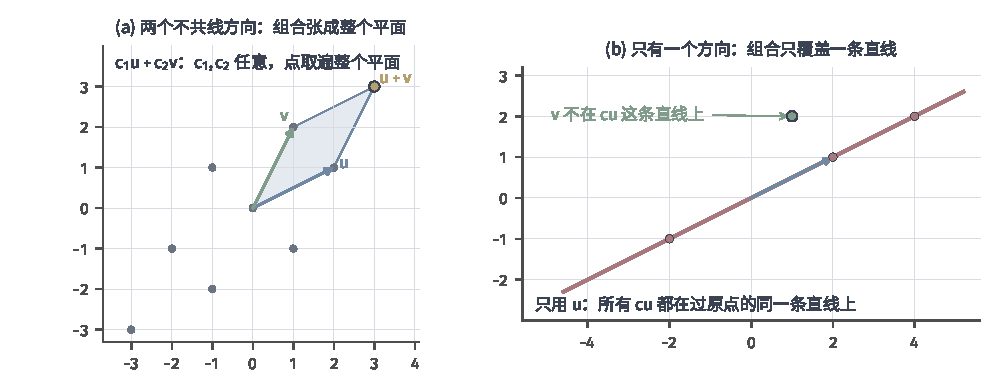
\includegraphics[width=169mm]{figures/01-mathematical-preliminaries-upper/02-linear-spaces/matplotlib/ls-linear-combination-span/ls-linear-combination-span.pdf}
  \caption{两个方向与一个方向的张成范围。左：$\bm u=(2,1)$（蓝箭头）与$\bm v=(1,2)$（绿箭头）的全部加权组合取遍整个平面，浅蓝平行四边形标出$0,\bm u,\bm u+\bm v,\bm v$，灰点为整数系数格点，黄点为$\bm u+\bm v=(3,3)$。右：只有$\bm u$一个方向时，组合$\{c\bm u\}$只是过原点的一条直线（红线），$\bm v$不在其上。两图坐标等比例，为解析教学例。}
  \label{fig:ls-linear-combination-span}
\end{figure*}

\paragraph{零向量的表示与线性无关}
表示是否冗余，要看零向量能否被非平凡地表示。若
\begin{equation}
 a_1\bm v_1+\cdots+a_k\bm v_k=\bm0
 \label{eq:linear-algebra-independence-relation}
\end{equation}
仅在全部$a_j=0$时成立，就称这组向量\term{线性无关}（linearly independent）；
否则称为\term{线性相关}（linearly dependent），即存在不全为零的系数使式
\eqref{eq:linear-algebra-independence-relation}成立。线性相关时挑出一个非零
系数$a_j$并移项，就能把$\bm v_j$写成其余向量的线性组合，说明这个方向重复了
已有方向能到达的范围。

在贯穿例\eqref{eq:linear-algebra-nearly-collinear-design}中，
$a_1\bm c_1+a_2\bm c_2=(a_1+a_2)\bm c_1+a_2\varepsilon\bm q$。
$\bm c_1$与$\bm q$线性无关，所以$\varepsilon\neq0$时两个系数只能都为零；
$\varepsilon=0$时却有$\bm c_1-\bm c_2=\bm0$。因此近共线和线性无关不同：
前者描述接近退化的程度，后者是精确的是非判断。

“能表示哪些对象”和“表示是否冗余”是两个独立的问题，分别由张成与线性无关回答。
在$\mathbb R^2$中取$\bm v_1=(1,0)^{\top}$、$\bm v_2=(0,1)^{\top}$，
$a_1\bm v_1+a_2\bm v_2=(a_1,a_2)^{\top}$可以取到平面上每个点，系数被目标点
唯一确定，这是“足够且无冗余”。只取$\bm v_1$一组方向，能到达的只是一条直线，
张成不够；再把$\bm v_3=(1,1)^{\top}$加入前两组，能到达的点仍只是整个平面，
$(1,1)^{\top}$却有$a_1=a_2=0,a_3=1$与$a_1=a_2=1,a_3=0$两组系数，这是
张成足够但表示冗余。图~\ref{fig:vol1-add-linear-redundant-directions}把这两种
表示画到同一个平面上。
\begin{figure}[!htb]
  \centering
  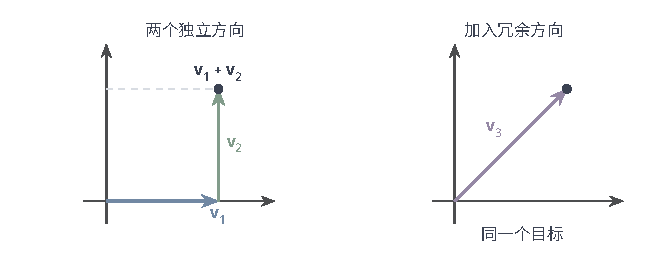
\includegraphics[width=112mm]{figures/01-mathematical-preliminaries-upper/02-linear-spaces/tikz/comprehension-additions/linear-redundant-directions.pdf}
  \caption{冗余方向与重复表示。取$\bm v_1=(1,0)^{\top}$、$\bm v_2=(0,1)^{\top}$与$\bm v_3=(1,1)^{\top}$。左图沿$\bm v_1$再沿$\bm v_2$，右图直接沿$\bm v_3$，到达同一个目标；前两向量已能表示平面中的每个向量，加入$\bm v_3$只使生成组冗余。两图坐标等比例。}
  \label{fig:vol1-add-linear-redundant-directions}
\end{figure}
存在性来自张成：张成之内的对象必有一组系数。唯一性来自线性无关：若同一对象
有两组系数，相减得到式\eqref{eq:linear-algebra-independence-relation}，
无关性保证两组系数完全相同。

反过来，唯一性也蕴含无关性。若存在一组不全为零的系数使线性组合为零，把这组
系数加到某个对象的一组表示上，就得到同一对象的第二组表示，表示不再唯一。
所以“张成内每个对象的系数唯一”与“零向量只有平凡表示”是同一件事的两面，
这正是后面坐标定义可以放心使用的根据。

\subsection{基与维数}
\label{sec:ls-basis-dimension}

\paragraph{基的抽取与扩充}
张成保证表示存在，无关保证表示唯一；同时做到这两条的一组向量，就是整个空间的
一把“尺子”。同时满足张成和线性无关的一组向量称为\term{基}（basis）：它足够
到达整个空间，又不重复。从任一有限生成组中反复抽取：若某成员能写成其余向量的
线性组合，删去它不会缩小张成范围，继续检查直到剩下的向量两两不可由其余表示，
最终得到一组线性无关的生成向量，即基。反过来，任一线性无关组可以逐次加入不在
其张成空间中的向量，直至扩充成基：每加入一个新方向，张成范围严格扩大；有限
空间迟早被填满，停止时留下的就是基。两条路线互补：抽取把冗余生成组压成基，
扩充把无关组补成基。

\paragraph{维数}
基的向量个数称为空间的\term{维数}（dimension）$\dim V$。这里有一个必须
先回答的问题：换一组基，个数会不会变？答案由交换引理给出。
\begin{theorem}[交换引理]
\label{thm:ls-exchange-lemma}
若$\bm u_1,\ldots,\bm u_r$线性无关，且每个$\bm u_i$都属于
$\operatorname{span}\{\bm v_1,\ldots,\bm v_s\}$，则$r\leq s$；并且这$r$个
$\bm u_i$可以逐个换入原生成组、换出同样多个$\bm v_j$，每次换完新组仍张成
原来的空间。
\begin{proof}
从生成组$G_0=\{\bm v_1,\ldots,\bm v_s\}$开始。因为$\bm u_1\in\operatorname{span}G_0$，
它可写成若干$\bm v_j$的组合；这些系数不能全为零，否则$\bm u_1=\bm0$，与
$\bm u_1,\ldots,\bm u_r$线性无关矛盾。取某个系数非零的$\bm v_j$，把它解出来：
$\bm v_j$可由$\bm u_1$与其余$\bm v$的组合表示，于是用$\bm u_1$换出$\bm v_j$，
新组$G_1$与$G_0$张成同一个空间。

一般地，第$i-1$步后的组$G_{i-1}$由$\bm u_1,\ldots,\bm u_{i-1}$和
$s-(i-1)$个幸存的$\bm v$组成，且与$G_0$张成同一空间。于是
$\bm u_i\in\operatorname{span}G_{i-1}$。若$\bm u_i$只用
$\bm u_1,\ldots,\bm u_{i-1}$就能表示，它与前面$i-1$个方向重复，违反
线性无关；所以表达式中至少一个幸存$\bm v$的系数非零，把它解出并换入
$\bm u_i$，张成范围不变。只要还有幸存$\bm v$，这一步就能做下去。

若$r>s$，换满$s$次以后组内只剩$\bm u_1,\ldots,\bm u_s$，却仍有
$\bm u_{s+1}$待入列；它属于$\operatorname{span}G_s=\operatorname{span}\{\bm u_1,\ldots,\bm u_s\}$，
与$r$个$\bm u$线性无关矛盾。故$r\leq s$，而上面的逐次交换正是定理要求的
换入换出过程。
\end{proof}
\end{theorem}

由此维数才是良定义的。任取两组基：把第一组看成无关组、第二组看成生成组，得
$r\leq s$；互换两组的角色又得$s\leq r$，所以$r=s$，换基不改变基的个数。
只含零向量的空间允许空基，维数为$0$。这一有限维结论支持后面的基扩充与维数
计算，不直接推广到无限维函数展开。$\mathbb R^d$的标准基
$\bm e_1,\ldots,\bm e_d$（第$j$个坐标为$1$、其余为$0$）是一组基，故
$\dim\mathbb R^d=d$；$P_k$的基为$1,t,\ldots,t^k$，故$\dim P_k=k+1$。

\section{子空间}
\label{sec:ls-subspaces}
\label{sec:linear-algebra-relations}
\label{sec:linear-algebra-subspace-relations}

固定同一个有限维实空间$V$，本节研究它的子空间怎样包含、相交与组合：包含比较
两个范围的大小，交找出公共方向，和合并两组方向，直和进一步要求分解唯一。这里
比较的始终是同一环境中的线性范围，不涉及长度或夹角。

\subsection{子空间包含}
\label{sec:ls-subspace-inclusion}

若子空间$U$的每个元素都属于子空间$W$，就记$U\subseteq W$。包含比较的是对象
范围：$U$的全部方向都在$W$中。取$U$的一组基，它在$W$中仍线性无关，按
~\ref{sec:ls-basis-dimension}节的基扩充补成$W$的基；只要$U$不占满$W$，
新增方向就不会是空的，因此$\dim U\leq\dim W$。

包含且同维，结论立刻收紧为相等。$\dim U=\dim W$时，$U$的基扩充成$W$的基
不需要新增任何方向，它本身已经张成$W$，故$U=W$。

反过来，同维本身推不出包含。平面中的两条不同直线维数都是$1$，却互不包含：
维数只数方向的个数，不管这些方向具体指向哪里。

把$U$的基扩充为$W$的基时，新增方向的个数恰为$\dim W-\dim U$，记录
$U$之外还有多少自由度。后面核与像、商空间的维数计算，都复用这一“先取已有基、
再补新方向”的做法。

\subsection{交空间}
\label{sec:ls-intersection}

两个子空间$U,W\subseteq V$的交$U\cap W$由同时属于二者的元素组成。它仍是
子空间：$\bm x,\bm y\in U\cap W$时二者既在$U$也在$W$，故$a\bm x+b\bm y$
同属两边。

交也是同时包含在$U$与$W$中的最大子空间：任何想同时装下两边公共方向的子空间，
装下的只能是交里的元素。平面中的画面帮着理解：两条重合的直线交出整条直线；
两条不同直线只交出零子空间。交为零只说明没有公共的非零方向，并不声称二者
合起来覆盖整个平面。

当$U,W$分别由齐次线性约束描述时，交就是同时满足两组约束的解集合。例如
$U=\{\bm x:x_1=0\}$与$W=\{\bm x:x_2=0\}$的交是
$\{\bm x:x_1=x_2=0\}$。集合与约束的对应在这里建立，具体消元求基留到求解章。

\subsection{和空间}
\label{sec:ls-sum}

\paragraph{维数公式}
两组方向联合能到达的对象组成和空间
$U+W=\{\bm u+\bm w:\bm u\in U,\ \bm w\in W\}$。它对线性组合封闭，是同时
包含$U,W$的最小子空间。注意并集$U\cup W$一般不对相加封闭，和空间补入了必要的
线性组合。

先取$U\cap W$的一组基，分别扩充为$U$与$W$的基；两组新增方向与共有基合起来
张成$U+W$。若其线性组合为零，把$U$一侧移到$W$一侧便得到交中的向量，各自
扩充基的无关性迫使新增系数为零，共有系数也为零。因此
\begin{equation}
 \dim(U+W)=\dim U+\dim W-\dim(U\cap W).
 \label{eq:ls-dimension-formula}
\end{equation}
被减去的维数正是两边重复计入的公共方向，而不是两个集合元素个数的差。例如在
$\mathbb R^3$中$U=\operatorname{span}\{\bm e_1,\bm e_2\}$、
$W=\operatorname{span}\{\bm e_2,\bm e_3\}$，交为$\operatorname{span}\{\bm e_2\}$，
$\dim(U+W)=3=2+2-1$；若把两条不同坐标轴当作$U,W$，交为零，和的维数直接相加。

\subsection{直和}
\label{sec:ls-direct-sum}

\paragraph{补空间}
平面上一条直线只能记录部分方向；再取一条不平行的直线，平面中的每个向量就能
拆成两个部分，各占一条直线上的一份。把这种“分解唯一”的要求写成代数条件：
若$U\cap W=\{\bm0\}$，则$U+W$中每个向量的两部分分解唯一：若
$\bm u_1+\bm w_1=\bm u_2+\bm w_2$，移项得$\bm u_1-\bm u_2=\bm w_2-\bm w_1$，
左边在$U$、右边在$W$，故同属交，只能是零，于是$\bm u_1=\bm u_2$、
$\bm w_1=\bm w_2$。这时称和为\term{直和}（direct sum），记为$U\oplus W$。
唯一分解不要求正交：平面中的两条非平行直线就构成直和，实际写出分量还要选择
相应基。

要写$V=U\oplus W$，还须满足$U+W=V$，这样的$W$称为$U$在$V$中的
\term{补空间}（complement）。
有限维中由基扩充总能选出这样的$W$，但选择一般不唯一：在平面中给一条直线选补空间，
任何不平行于它的直线都可以。指定内积以后的正交补是另一回事，由内积一节介绍，
不能把一般补空间自动称为正交补。

\section{坐标与换基}
\label{sec:ls-coordinates-change-of-basis}
\label{sec:linear-algebra-coordinate-conversions}

基保证表示唯一以后，本节研究怎样从基读出坐标，以及换一组基时同一对象的记录怎样
转换。被动换基只改变记录方式，不是对对象施加新的作用。

\subsection{坐标}
\label{sec:ls-coordinates}
\label{sec:linear-algebra-coordinates}

固定有序基$\mathcal B=(\bm b_1,\ldots,\bm b_d)$后，对象$\bm v$唯一写成
$\sum_{j=1}^d x_j\bm b_j$。系数列
$[\bm v]_{\mathcal B}=(x_1,\ldots,x_d)^{\top}$称为$\bm v$在基$\mathcal B$
下的\term{坐标}（coordinates）。存在性来自张成，唯一性来自线性无关，所以坐标
映射$\bm v\mapsto[\bm v]_{\mathcal B}$是线性双射。如图~\ref{fig:ls-basis-coordinates}
所示，同一个几何向量在标准基下读出$(1,2)$，在斜基$\bm b_1=(2,1)$、
$\bm b_2=(-1,1)$下读出$(1,1)$：向量本身没有移动，只是沿不同的基尺子去量。
\begin{figure*}[htbp]
  \centering
  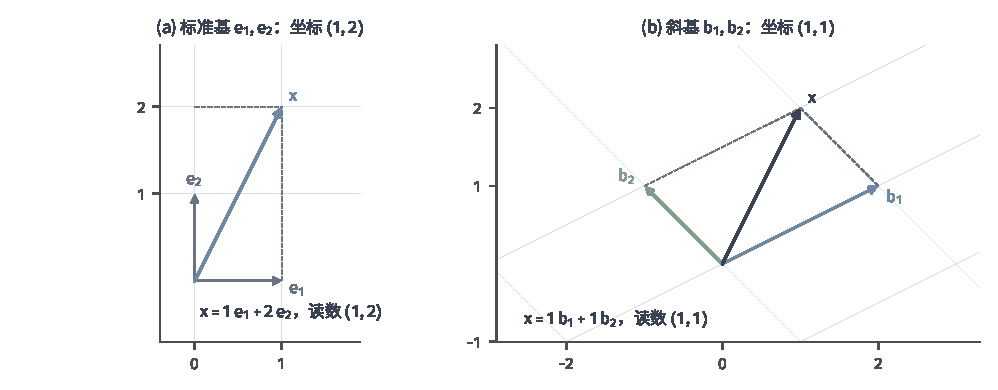
\includegraphics[width=169mm]{figures/01-mathematical-preliminaries-upper/02-linear-spaces/matplotlib/ls-basis-coordinates/ls-basis-coordinates.pdf}
  \caption{同一向量在两组基下的坐标。左：标准基$\bm e_1,\bm e_2$（灰箭头）下，向量$\bm x=(1,2)$（蓝箭头）的坐标为$(1,2)$，虚线为向坐标轴的垂线。右：斜基$\bm b_1=(2,1)$（蓝）、$\bm b_2=(-1,1)$（绿）下，同一个$\bm x$满足$\bm x=\bm b_1+\bm b_2$，坐标为$(1,1)$，浅色斜线为斜基网格，虚线为平行四边形读法。两图坐标系相同。}
  \label{fig:ls-basis-coordinates}
\end{figure*}

基的顺序同时固定：交换$\bm b_1,\bm b_2$，对象不变，坐标列的前两个数也交换。
在$\mathbb R^d$中直接写数字列，通常是默认使用标准基$\bm e_1,\ldots,\bm e_d$。
函数基展开完全如此：函数是对象，展开系数是坐标，例如$f_{a,b}=a\cdot1+b\cdot t$
在基$(1,t)$下的坐标是$(a,b)^{\top}$。坐标个数是维数，不能由某个冗余记录的
长度直接推断。

对象不变时，坐标仍可能很不一样。固定$\delta=0.1$并令
\begin{equation}
 \bm y=\bm c_1+\delta\bm q=\begin{bmatrix}1\\1.1\\0.9\end{bmatrix}.
 \label{eq:linear-algebra-nearly-collinear-target}
\end{equation}
在$\mathcal B_0=(\bm c_1,\bm q)$下坐标是$(1,\delta)^{\top}$。若
$\varepsilon\neq0$，改用同一平面上的基$\mathcal B_\varepsilon=(\bm c_1,\bm c_2)$，
则
\begin{equation}
 \bm y=\left(1-\frac{\delta}{\varepsilon}\right)\bm c_1
       +\frac{\delta}{\varepsilon}\bm c_2.
 \label{eq:linear-algebra-coordinate-instability}
\end{equation}
$\varepsilon=0.01$时坐标成为$(-9,10)^{\top}$，但$\bm y$没有改变。两个很大的
系数在几乎同向的基向量上相消，不能据此判断原对象很大；这种系数对基接近退化的
敏感，将在误差分析章定量讨论。

\subsection{换基}
\label{sec:ls-change-basis}

设$\mathcal C$是另一组基。把各$\bm b_j$的$\mathcal C$坐标排成列，得到换基矩阵
$\bm S_{\mathcal C\leftarrow\mathcal B}$；保持线性组合给出
\begin{equation}
 [\bm v]_{\mathcal C}
 =\bm S_{\mathcal C\leftarrow\mathcal B}[\bm v]_{\mathcal B}.
 \label{eq:linear-algebra-coordinate-change}
\end{equation}
沿反方向换基能恢复原坐标，两个坐标变换互逆。在贯穿例中，
$\bm S_{\mathcal B_0\leftarrow\mathcal B_\varepsilon}
=\begin{bmatrix}1&1\\0&\varepsilon\end{bmatrix}$，反向求坐标要除以
$\varepsilon$，已提示小扰动可能被放大。此处改变的是记录方式，不是对对象施加
新的物理变换。图~\ref{fig:vol1-add-linear-change-basis}核对了这种区别：目标
位置没有移动，改变的只是沿哪两条基方向累加，以及每条方向取多少份。
\begin{figure}[!htb]
  \centering
  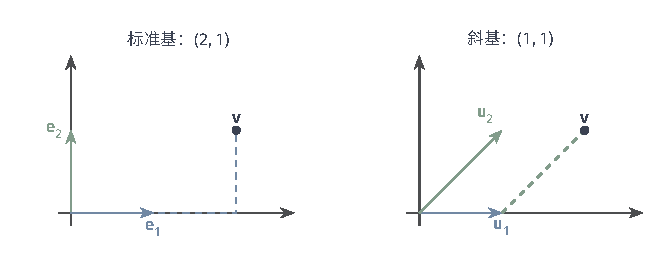
\includegraphics[width=112mm]{figures/01-mathematical-preliminaries-upper/02-linear-spaces/tikz/comprehension-additions/linear-change-basis.pdf}
  \caption{同一向量的两套坐标。左图使用标准基，$\bm v=(2,1)^{\top}$的坐标为$(2,1)^{\top}$；右图使用$\bm c_1=(1,0)^{\top}$、$\bm c_2=(1,1)^{\top}$，同一$\bm v$的坐标为$(1,1)^{\top}$。虚线表示相应的向量相加，两图的环境坐标比例相同。}
  \label{fig:vol1-add-linear-change-basis}
\end{figure}

若再换到第三组基$\mathcal D$，中间坐标应相消：
$\bm S_{\mathcal D\leftarrow\mathcal B}
=\bm S_{\mathcal D\leftarrow\mathcal C}\bm S_{\mathcal C\leftarrow\mathcal B}$。
这是逐坐标代入的结果：先按$\mathcal B$读出$\bm v$，再用$\mathcal C$坐标表示，
最后换到$\mathcal D$，中间那套坐标不留下痕迹。

被动换基与主动作用必须分开。换基时对象不动、记录改变，式
\eqref{eq:linear-algebra-coordinate-change}两侧是同一个$\bm v$的两套坐标；
主动作用则是固定坐标把对象送到另一个对象，例如把向量旋转或缩放。图
~\ref{fig:ls-passive-change-vs-active-map}把两种情形并排放置：左图中向量位置
不动，读数从$(3,3)$变成$(2,1)$；右图中坐标系不动，向量$\bm x=(3,3)$被切变
$\bm A=\begin{bmatrix}1&1\\0&1\end{bmatrix}$搬到$\bm A\bm x=(6,3)$。两者
乘法形式相似，含义不同，不能把所有乘矩阵都理解成换基；主动作用在
~\ref{sec:ls-linear-maps}节作为线性映射建立。
\begin{figure*}[htbp]
  \centering
  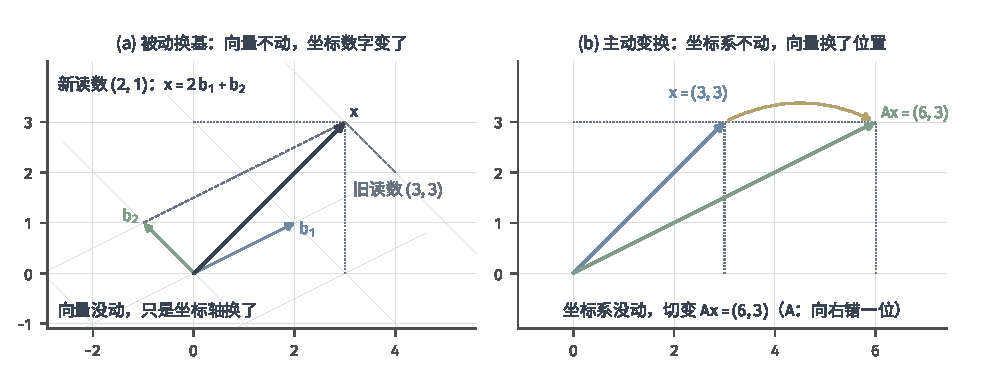
\includegraphics[width=169mm]{figures/01-mathematical-preliminaries-upper/02-linear-spaces/matplotlib/ls-passive-change-vs-active-map/ls-passive-change-vs-active-map.pdf}
  \caption{被动换基与主动变换的对照，两图使用同一个初始向量$\bm x=(3,3)$。左（被动换基）：箭头位置不动（深色），旧标准读数用点线投影读出$(3,3)$；新斜基$\bm b_1=(2,1)$（蓝）、$\bm b_2=(-1,1)$（绿）与浅色斜网格下，$\bm x=2\bm b_1+\bm b_2$，新读数为$(2,1)$。右（主动变换）：标准坐标系不动，$\bm x$（蓝）被切变映到$\bm A\bm x=(6,3)$（绿），黄色弧线表示搬动过程。}
  \label{fig:ls-passive-change-vs-active-map}
\end{figure*}

\section{线性映射}
\label{sec:ls-linear-maps}
\label{sec:linear-algebra-matrices-linear-maps}

对象之间的作用怎样决定输出、又保留或丢失了哪些输入信息，是本节的问题。选定输入与
输出两端的基以后，作用被记录为矩阵；核、像与秩零度定理描述被消去和被保留的
自由度，并据此判断何时可以由输出反求输入。

\subsection{线性映射}
\label{sec:ls-linear-map-definition}
\label{sec:linear-algebra-maps}

保持线性组合的作用称为\term{线性映射}（linear map）$T:V\to W$：
\begin{equation}
 T(a\bm x+b\bm y)=aT\bm x+bT\bm y,
 \qquad \bm x,\bm y\in V,\ a,b\in\mathbb R.
 \label{eq:ls-linear-map-def}
\end{equation}
特别有$T\bm0=\bm0$。第~\ref{chap:sets-functions-and-proofs}章
~\ref{sec:prelim-linear-actions-composition}节已经看到
矩阵乘向量满足这条规则，这里把它作为作用的一般定义。

给定输入基$\mathcal B=(\bm b_1,\ldots,\bm b_d)$和输出基$\mathcal C$，只要
记录每个基向量的像就能记录整个映射：由线性性，$T(\sum_j x_j\bm b_j)
=\sum_j x_jT\bm b_j$。把$[T\bm b_j]_{\mathcal C}$作为第$j$列，得到矩阵
$\bm A=[T]_{\mathcal C\leftarrow\mathcal B}\in\mathbb R^{m\times d}$，并有
\begin{equation}
 [T\bm v]_{\mathcal C}
 =[T]_{\mathcal C\leftarrow\mathcal B}[\bm v]_{\mathcal B}
 =\bm A[\bm v]_{\mathcal B}.
 \label{eq:linear-algebra-map-matrix-representation}
\end{equation}
列数是输入维数，行数是输出维数。图~\ref{fig:ch06-object-coordinate-map}中两条
路径给同一结果，表明矩阵是映射在两端坐标下的表示，不是映射本身的全部含义：改变
两端任一组基通常改变数表，却仍记录同一个映射。
\begin{figure}[htbp]
  \centering
  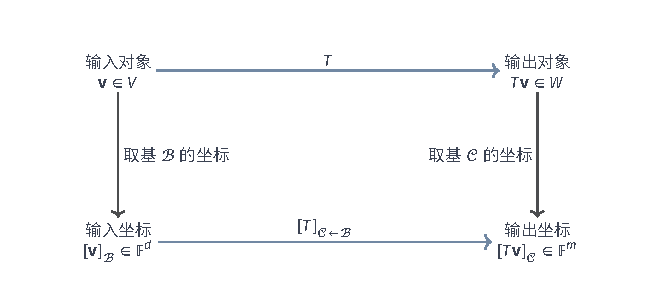
\includegraphics[width=112.0mm]{figures/01-mathematical-preliminaries-upper/02-linear-spaces/tikz/ch06-object-coordinate-map/figure.pdf}
  \caption{先作用于对象再取坐标，与先取输入坐标再乘矩阵，得到相同输出坐标。横向箭头改变对象或数值，竖向箭头只改变记录方式。}
  \label{fig:ch06-object-coordinate-map}
\end{figure}

设计矩阵$\bm X_\varepsilon$表示$T_\varepsilon:\mathbb R^2\to\mathbb R^3$，
$\bm w\mapsto w_1\bm c_1+w_2\bm c_2$。输入是两个系数，输出是三个样本的拟合值，
二者不能当成同一个空间中的向量。

带常数偏置的规则$\bm x\mapsto\bm A\bm x+\bm b$在$\bm b\neq\bm0$时为
\term{仿射映射}（affine map），不是线性映射：它把$\bm0$送到$\bm b$，而线性
映射必将$\bm0$送到$\bm0$。增广坐标
\begin{equation*}
 \begin{bmatrix}\bm A&\bm b\\\bm0^{\top}&1\end{bmatrix}
 \begin{bmatrix}\bm x\\1\end{bmatrix}
 =\begin{bmatrix}\bm A\bm x+\bm b\\1\end{bmatrix}
\end{equation*}
对增广空间是线性的，但原输入被限制在末坐标为$1$的仿射集合上，不能因此声称原映射
线性。仿射解集的几何在求解章直接使用这一形式。

\subsection{核与像}
\label{sec:ls-kernel-image}

被送到零的输入集合称为\term{零空间}（核，kernel）：
$\ker T=\{\bm x\in V:T\bm x=\bm0\}$；所有可到达的输出集合称为\term{像空间}
（像，image）：$\operatorname{im}T=\{T\bm x:\bm x\in V\}$。二者都是子空间：
若$T\bm x=T\bm y=\bm0$，则$T(a\bm x+b\bm y)=\bm0$；若$\bm u=T\bm x$、
$\bm v=T\bm y$，则$a\bm u+b\bm v=T(a\bm x+b\bm y)$。核记录被映射完全消去的
独立输入方向，像记录可达的输出范围；二者分别位于输入端与输出端，不能当作同一空间
中的两个集合直接比较。

例如用三个响应读取四个分量，教学矩阵$\bm S=[\,\bm I_3\mid\bm1\,]$满足
$\bm S(1,1,1,1)^{\top}=\bm S(0,0,0,2)^{\top}=(2,2,2)^{\top}$。两输入之差
$(1,1,1,-1)^{\top}$在核中，所以仅凭响应无法区分它们。这演示的是线性不可辨识性：
两个输入相差核方向时输出相同，具体约束下的合法输入范围另有限制。

\subsection{秩与零度}
\label{sec:ls-rank-nullity}

\paragraph{秩零度定理与独立约束}
像的维数称为\term{秩}（rank）$\operatorname{rank}T=\dim\operatorname{im}T$，
核的维数称为\term{零度}（nullity）$\dim\ker T$。
\begin{theorem}[秩零度定理]
\label{thm:ls-rank-nullity}
\label{thm:linear-algebra-rank-nullity}
有限维线性映射$T:V\to W$满足
\begin{equation}
 \dim V=\dim\ker T+\dim\operatorname{im}T,
 \qquad\text{即}\qquad
 \dim V=\dim\ker T+\operatorname{rank}T.
 \label{eq:ls-rank-nullity}
\end{equation}
\end{theorem}
\begin{proof}
取核的一组基$\bm v_1,\ldots,\bm v_r$并扩充成$V$的基
$\bm v_1,\ldots,\bm v_d$。前$r$个基向量的像为零，所以其余像
$T\bm v_{r+1},\ldots,T\bm v_d$张成像。若$\sum_{j>r}a_jT\bm v_j=\bm0$，
则$\sum_{j>r}a_j\bm v_j$属于核，能由前$r$个基向量表示；整个基的线性无关性
迫使全部$a_j=0$，所以这些像也是无关组。像的维数为$d-r$，结论成立。
\end{proof}
对矩阵$\bm A\in\mathbb R^{m\times d}$，记$\operatorname{rank}\bm A$为其映射
的秩，有$d=\dim\ker\bm A+\operatorname{rank}\bm A$。秩计数独立的输出方向，
零度计数被消去的独立输入方向，二者此消彼长。图
~\ref{fig:ls-kernel-image-rank-nullity}给出两个几何化算例：被映到零的方向与
实际用到的输出方向，维数相加恰为定义域维数。
\begin{figure*}[htbp]
  \centering
  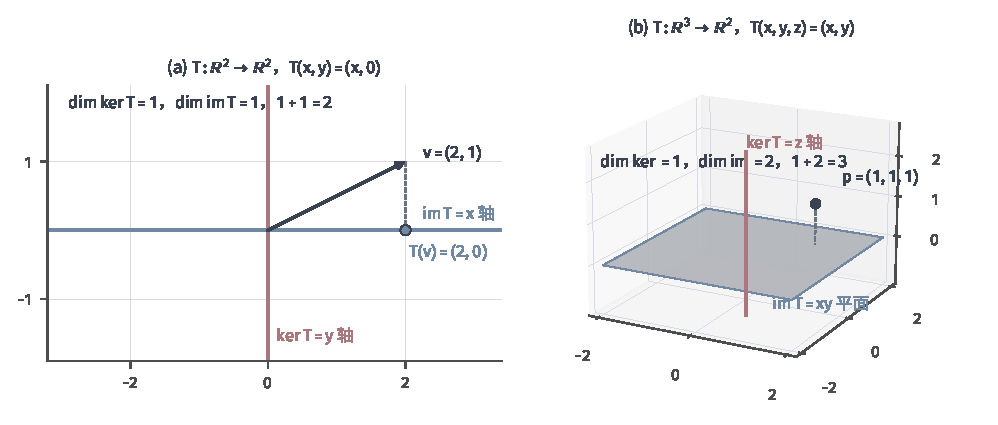
\includegraphics[width=169mm]{figures/01-mathematical-preliminaries-upper/02-linear-spaces/matplotlib/ls-kernel-image-rank-nullity/ls-kernel-image-rank-nullity.pdf}
  \caption{核与像的维数此消彼长。左：$T(x,y)=(x,0)$把平面映到$x$轴，核是$y$轴（红直线）、像是$x$轴（蓝直线），$\dim\ker T=1$、$\dim\operatorname{im}T=1$，$1+1=2$；样本$\bm v=(2,1)$被映到$(2,0)$。右：$T(x,y,z)=(x,y)$把三维空间映到$xy$平面，核是$z$轴（红直线）、像是整个$xy$平面（浅蓝），$\dim\ker T=1$、$\dim\operatorname{im}T=2$，$1+2=3$。两图为解析教学例。}
  \label{fig:ls-kernel-image-rank-nullity}
\end{figure*}

对$\bm A\in\mathbb R^{m\times d}$，$\operatorname{rank}\bm A\leq\min(m,d)$。
$\operatorname{rank}\bm A=d$称为满列秩，输入方向全部被保留；
$\operatorname{rank}\bm A=m$称为满行秩，输出全部可达；二者统称
\term{满秩}（full rank）。形状不同时二者不能
同时成立：$m<d$时满行秩仍可能有非零核，$m>d$时满列秩仍可能有输出缺失。
这里以列张成空间读取秩；行秩等于列秩的证明在~\ref{sec:ls-dual-map}节由对偶
映射补齐。

\subsection{单射、满射与可逆性}
\label{sec:ls-injective-surjective-invertible}
\label{sec:prelim-inverse-matrices}

\paragraph{逆与单侧逆}
第~\ref{chap:sets-functions-and-proofs}章~\ref{sec:prelim-function-types}节按一般
函数定义过单射、满射与双射。对线性
映射，单射等价于核为零：$T\bm x=T\bm y$当且仅当$\bm x-\bm y\in\ker T$，
核为零时输出相同必输入相同。满射等价于像等于整个输出空间。二者同时成立时得到
线性双射，每个输出恰有一个原输入，逆映射$T^{-1}:W\to V$也是线性的。有限维且
输入输出维数相等时，秩零度定理给出单射、满射、双射等价；维数不同则须分别判断，
不把矩形矩阵的满秩直接说成双侧可逆。

对$n$阶方阵$\bm A$，若存在$n$阶方阵$\bm B$满足
$\bm A\bm B=\bm B\bm A=\bm I_n$，就称$\bm A$可逆，$\bm B$为
\term{逆矩阵}（inverse matrix），记作$\bm A^{-1}$。两边的单位矩阵条件分别
保证先后两个方向的乘法都能撤销。若$\bm B,\bm C$都满足条件，则
\[
 \bm B=\bm B\bm I_n=\bm B(\bm A\bm C)
 =(\bm B\bm A)\bm C=\bm I_n\bm C=\bm C,
\]
所以逆矩阵唯一，每次改写只使用结合律，没有交换矩阵次序。

可逆要回答的问题是：给一个输出，能否唯一还原输入。先看最容易还原的情形——
对角矩阵把各坐标分别乘以一个数，坐标之间互不影响，撤销它就是逐坐标除以这些
数。每个$d_i\neq0$时，
$\operatorname{diag}(d_1,\ldots,d_n)^{-1}
=\operatorname{diag}(1/d_1,\ldots,1/d_n)$，例如
$\operatorname{diag}(2,1)$的逆为$\operatorname{diag}(1/2,1)$。

这一简单情形同时划出不可逆的边界：若某个$d_i=0$，相应坐标被压为零，两个只在
该坐标不同的输入给出相同输出，反求必然失败。对角情形把“可逆等于每个输入方向
都能被原样读回”看得最清楚；一般矩阵把坐标掺在一起，不能逐坐标处理，但撤销
的目标相同：对一般可逆矩阵，$\bm A\bm x=\bm y$左乘$\bm A^{-1}$，得到唯一的
$\bm x=\bm A^{-1}\bm y$。

两个可逆方阵接连作用时，撤销过程应当倒过来执行，这与逆映射的复合规则相同：
若$\bm A,\bm B$都是$n$阶可逆方阵，则
\begin{equation}
 (\bm A\bm B)^{-1}=\bm B^{-1}\bm A^{-1}.
 \label{eq:ls-inverse-product}
\end{equation}
验证：$(\bm A\bm B)(\bm B^{-1}\bm A^{-1})
=\bm A(\bm B\bm B^{-1})\bm A^{-1}=\bm I_n$，反方向也等于单位矩阵。这里的
逆一般不是逐元素取倒数；矩阵乘法的行列混合决定了它必须作为整体计算。

矩形矩阵没有方阵意义的双侧逆。满列秩的长矩阵可有左逆$\bm L$使
$\bm L\bm A=\bm I_d$，满行秩的宽矩阵可有右逆$\bm R$使$\bm A\bm R=\bm I_m$，
但这些单侧逆一般不唯一。此处只判断恢复关系是否存在；如何通过分解应用逆、多解时
如何选择代表，分别由运算章与求解章回答。

\section{对偶空间}
\label{sec:ls-dual-spaces}

怎样把一个对象线性地读成一个数，读取规则又怎样随映射改变？本节从线性泛函构造对偶
基，再由复合定义对偶映射并给出转置表示；这一代数构造不依赖长度、夹角或内积，
内积意义下的伴随在运算章建立。

\subsection{对偶空间}
\label{sec:ls-dual-space}

读取多项式在$t=0$处的取值、取信号的第一个样本、计算一组系数加权和，都是把一个
对象读成一个数。保持线性组合的标量读取称为\term{线性泛函}（linear functional）：
$\varphi:V\to\mathbb R$满足$\varphi(a\bm x+b\bm y)
=a\varphi(\bm x)+b\varphi(\bm y)$。读取一个坐标、计算一个线性加权和都是
线性泛函；同一个对象可以接受多种读取。全部线性泛函按逐点加法与数乘
$(\alpha\varphi+\beta\psi)(\bm x)=\alpha\varphi(\bm x)+\beta\psi(\bm x)$
组成线性空间，称为$V$的\term{对偶空间}（dual space）$V^*$。输入向量是被读取
的对象，泛函是读取规则，二者属于不同类型。

\paragraph{对偶基}
对$V$的基$\mathcal B=(\bm b_1,\ldots,\bm b_d)$，逐个定义泛函
$\varphi_j\in V^*$使
\begin{equation}
 \varphi_j(\bm b_i)=\delta_{ji}
 =\begin{cases}1,&i=j,\\0,&i\neq j.\end{cases}
 \label{eq:ls-dual-basis-def}
\end{equation}
任意$\varphi\in V^*$都能唯一展开为$\varphi=\sum_j\varphi(\bm b_j)\varphi_j$：
两边在$\bm b_i$上取值即得系数，无关性由$\varphi_j$的取值约束保证。这组
$\varphi_1,\ldots,\varphi_d$称为$\mathcal B$的\term{对偶基}（dual basis），
因而$\dim V^*=d=\dim V$。坐标可逐项恢复：$x_j=\varphi_j(\bm v)$。
标准基$\bm e_j$的对偶基就是第$j$坐标投影$x_j$。换一组基，对偶基随之更换：
取$\bm b_1=(1,1)^{\top}$、$\bm b_2=(1,0)^{\top}$，解$\varphi_j(\bm b_i)=\delta_{ji}$
得$\varphi_1(x,y)=y$、$\varphi_2(x,y)=x-y$；读取规则随基改变，但$\dim V^*$
不变。图~\ref{fig:ls-dual-basis-readout}在平面中把这种逐项读取画出来：对偶
方向$\bm b^1,\bm b^2$分别只在一个基方向上读到$1$，其余读到$0$。
\begin{figure}[htbp]
  \centering
  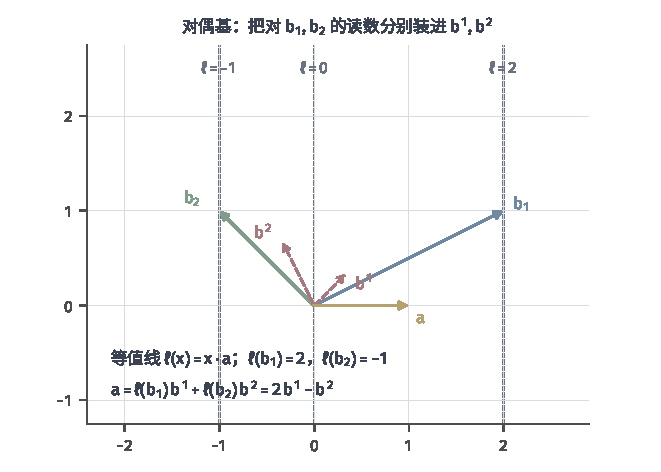
\includegraphics[width=112mm]{figures/01-mathematical-preliminaries-upper/02-linear-spaces/matplotlib/ls-dual-basis-readout/ls-dual-basis-readout.pdf}
  \caption{对偶读取的几何示意。蓝箭头$\bm b_1=(2,1)$、绿箭头$\bm b_2=(-1,1)$为基向量；红色虚线箭头为满足$\varphi_i(\bm b_j)=\delta_{ij}$的对偶基方向$\bm b^1=(1/3,1/3)$、$\bm b^2=(-1/3,2/3)$（本章中对偶基是读取规则；画成平面箭头借用的是内积意义下的对应向量，该对应在运算章建立）。黄色箭头$\bm a=(1,0)$给出读取$\ell(\bm x)=\bm a\cdot\bm x$，灰色虚线为等值线$\ell=c$（$c=-1,0,2$）；$\ell(\bm b_1)=2$、$\ell(\bm b_2)=-1$，且$\bm a=2\bm b^1-\bm b^2$。}
  \label{fig:ls-dual-basis-readout}
\end{figure}

\subsection{对偶映射}
\label{sec:ls-dual-map}

已知$T:V\to W$和输出端的读取$f\in W^*$，输入$\bm x$经过$T$后被读成
$f(T\bm x)$。由这项复合定义\term{对偶映射}（dual map）$T':W^*\to V^*$，
\begin{equation}
 T'f=f\circ T,\qquad (T'f)(\bm x)=f(T\bm x),
 \label{eq:ls-dual-map-def}
\end{equation}
反向传递的是读取规则，并非对$T$求逆。$T'$保持线性组合。

设输入基$\mathcal B=(\bm b_1,\ldots,\bm b_d)$、输出基
$\mathcal C=(\bm c_1,\ldots,\bm c_m)$下$T$的矩阵为$\bm A$，即
$T\bm b_j=\sum_i a_{i,j}\bm c_i$，对应的对偶基分别为$\varphi_j^V$、
$\varphi_i^W$。取输出读取$f=\sum_i y_i\varphi_i^W$，则
\begin{equation*}
 (T'f)(\bm b_j)=f(T\bm b_j)
 =\sum_i y_i\varphi_i^W\left(\sum_k a_{k,j}\bm c_k\right)
 =\sum_i a_{i,j}y_i=(\bm A^{\top}\bm y)_j.
\end{equation*}
所以$T'f$在输入对偶基下的系数列为$\bm A^{\top}\bm y$，即对偶映射的矩阵是
\term{转置}（transpose）$\bm A^{\top}$。这一推导只使用线性性和坐标，不需要
长度、夹角或内积；内积把读取方向识别为某个向量的表示，由运算章另行建立。

$\ker T'$由在$\operatorname{im}T$上恒为零的读取组成。设$r=\operatorname{rank}T$，
在$\operatorname{im}T$上取基并扩充为$W$的基，相应对偶读取中只有$m-r$个在
$\operatorname{im}T$上为零，故$\dim\ker T'=m-r$。对$T'$应用秩零度定理，
$\operatorname{rank}T'=m-(m-r)=r=\operatorname{rank}T$。在矩阵记录下
$\operatorname{rank}(\bm A^{\top})=\operatorname{rank}\bm A$，即行秩等于
列秩，闭合了~\ref{sec:ls-rank-nullity}节留下的判据。

\section{商空间}
\label{sec:ls-quotient-spaces}

当相差某个子空间内方向的对象应视为同一结果时，怎样表示忽略差别以后剩余的信息？
本节以差属于子空间定义等价，验证类上的运算与代表元无关，由基扩充求维数，最后把
商空间与映射的像对应起来。

\subsection{等价类}
\label{sec:ls-equivalence-classes}
\label{sec:linear-algebra-equivalence-relations}

例如只读取仿射函数在$t=0$处的截距时，斜率不同的两个函数应当被视为同一结果：
它们在截距上没有区别。把这种“忽略指定方向”的直觉写成代数关系。设$U$是$V$的
子空间，规定$\bm x\sim\bm y$当且仅当$\bm x-\bm y\in U$。这是
第~\ref{chap:sets-functions-and-proofs}章~\ref{def:prelim-equivalence-relation}定义的
等价关系：$\bm x-\bm x=\bm0\in U$
给出自反性；$\bm x-\bm y\in U$蕴含$\bm y-\bm x\in U$给出对称性；
$(\bm x-\bm y)+(\bm y-\bm z)=\bm x-\bm z\in U$给出传递性。
$\bm x$的\term{等价类}（equivalence class）为
$\bm x+U=\{\bm x+\bm n:\bm n\in U\}$；两个类相等不要求当前选取的代表元相等，
只要求代表元之差落在$U$中。全部等价类把$V$划分成互不重叠的块。图
~\ref{fig:ls-quotient-equivalence-classes}把这一划分画出来：子空间$U$是
$x$轴，平面被一族平行于$U$的直线切成一条条等价类，同一条线上的任意两点之差
都落在$U$中。
\begin{figure}[htbp]
  \centering
  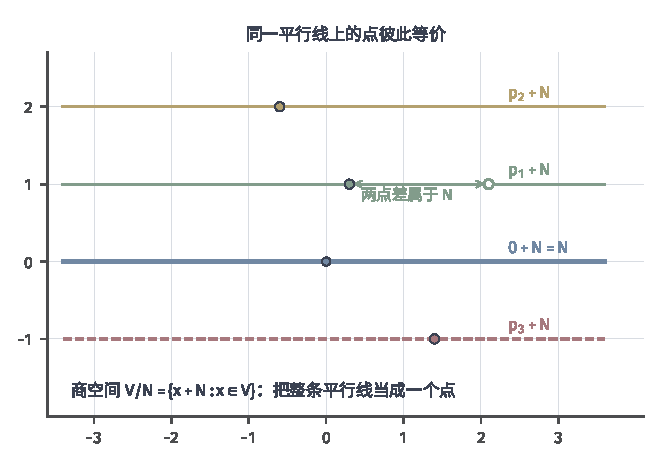
\includegraphics[width=112mm]{figures/01-mathematical-preliminaries-upper/02-linear-spaces/matplotlib/ls-quotient-equivalence-classes/ls-quotient-equivalence-classes.pdf}
  \caption{商空间的等价类。$V=\mathbb R^2$，子空间$U$为$x$轴（蓝线$0+U$）；每条平行直线$p+U=\{(x,p_y)\}$是一个等价类，图中画出$y=1$（绿）、$y=2$（黄）、$y=-1$（红虚线）。绿线上实点$(0.3,1)$与空心点$(2.1,1)$之差$(1.8,0)\in U$，故属同一类；商空间$V/U$把每条平行线当成一个点。}
  \label{fig:ls-quotient-equivalence-classes}
\end{figure}

\subsection{商空间}
\label{sec:ls-quotient-space}
\label{def:linear-algebra-quotient-space}

\paragraph{代表元无关}
全部等价类组成的集合$V/U$称为\term{商空间}（quotient space），其运算规定为
\begin{equation}
 (\bm x+U)+(\bm y+U)=(\bm x+\bm y)+U,
 \qquad
 a(\bm x+U)=a\bm x+U.
 \label{eq:ls-quotient-operations}
\end{equation}
换代表元$\bm x'=\bm x+\bm n_1$、$\bm y'=\bm y+\bm n_2$时，结果只相差
$\bm n_1+\bm n_2$或$a\bm n_1$，仍属于$U$，所以运算不依赖代表元。零类是
$U$本身，逆元为$-\bm x+U$，其余公理由$V$继承，$V/U$构成实线性空间。任务也
可以主动忽略一个指定子空间，不必先由误差尺度产生它；原对象、被忽略的方向和等价类
须分别记录。

取$U$的一组基$\bm u_1,\ldots,\bm u_s$并扩充为$V$的基
$\bm u_1,\ldots,\bm u_s,\bm v_1,\ldots,\bm v_t$。新增$\bm v_j$的等价类张成
$V/U$：任一$\bm x$写成两组基的组合，$U$部分落进零类被消去；这些类线性无关：
若$\sum_j a_j(\bm v_j+U)=U$，则$\sum_j a_j\bm v_j\in U$，它能由$\bm u_i$
表示，整个基的无关性迫使$a_j=0$。故商基有$t$个成员，
\begin{equation}
 \dim(V/U)=\dim V-\dim U.
 \label{eq:ls-quotient-dimension}
\end{equation}
例如仿射函数中只读取$t=0$处的截距时，零方向是$\operatorname{span}\{t\}$，
商空间只保留截距，被消去的是全部斜率方向。

\subsection{商映射}
\label{sec:ls-quotient-map}

自然映射$q:V\to V/U$把对象送到其等价类，$q(\bm x)=\bm x+U$。它线性：
$q(a\bm x+b\bm y)=(a\bm x+b\bm y)+U=a(\bm x+U)+b(\bm y+U)$，正是类上定义的
加法与数乘。它满射：$V/U$的每个类$\bm x+U$都有原代表$\bm x$。它的核恰为
$U$：$q(\bm x)=U$（零类）当且仅当$\bm x\in U$，即恰好被消去的方向组成这个
子空间。例如消去$\operatorname{span}\{t\}$后，截距类由$q(f_{a,b})=a+U$送出，
斜率$b$不在类中出现。

对$T:V\to W$取$U=\ker T$。规则$[\bm x]\mapsto T\bm x$不依赖代表元：
若$\bm x'=\bm x+\bm n$且$\bm n\in\ker T$，则$T\bm x'=T\bm x$。它线性、
满射到$\operatorname{im}T$，且核为零，因而是线性双射：
\begin{equation}
 V/\ker T\ \cong\ \operatorname{im}T.
 \label{eq:ls-first-isomorphism}
\end{equation}
压去全部丢失方向后，每个等价类恰对应一个可达输出；原映射本身未必具有双侧逆，
这里建立的是商空间与像之间的一一对应。

\section{矩阵表示的等价关系}
\label{sec:ls-matrix-equivalences}

不同矩阵是否记录同一个映射或同一个双线性读取？换基只改变记录、不改变对象，于是
同一对象在不同坐标下得到不同数表。本节分别在相似、相抵、合同内部讲清各自的坐标
约定、保持的不变量和验证条件，三者对象不同，不能混用。统一采用旧坐标
$\bm x=\bm P\bm x'$、$\bm y=\bm Q\bm y'$，带撇的是新坐标。本章只使用秩与
核维数等已经建立的量；迹、行列式的不变量在运算章相应定义后再补充，完整的实分裂
相似分类后置。

\subsection{相似}
\label{sec:ls-similarity}

\subsubsection{定义与含义}
\label{sec:ls-similarity-meaning}

同一个旋转，换一套坐标系以后写出来的数表并不相同；那么什么时候两个数表记录的是
同一个作用？固定同一个实线性自映射$T:V\to V$，比较它在两组基下的矩阵记录。
设旧基$\mathcal B$下坐标为$\bm x$，新基$\mathcal B'$下坐标为$\bm x'$，
旧矩阵$\bm A$满足$\bm y=\bm A\bm x$，新矩阵$\bm B$满足$\bm y'=\bm B\bm x'$。

旧坐标与新坐标由可逆换基矩阵联系：新基向量$\bm b_j'$在旧基下的坐标列拼成
$\bm P$的第$j$列，故对象的旧坐标$\bm x=\bm P\bm x'$，新坐标是旧坐标经
$\bm P$反向读出。$\bm P$可逆，因为两组基都能唯一表示$V$中的对象；反向
换基矩阵为$\bm P^{-1}$，把旧坐标换回新坐标。这里输入与输出是同一个空间、
同一组新基，所以输出坐标也按同一方式回换：$\bm y=\bm P\bm y'$。这是相似与
相抵的区别：相似两端使用同一次换基，$\bm P$左右两侧是同一个矩阵；相抵允许
输入、输出各自选基，左右两侧矩阵不同。

\paragraph{相似变换的推导}
把$\bm y=\bm P\bm y'$与$\bm x=\bm P\bm x'$代入$\bm y=\bm A\bm x$，得到
$\bm P\bm y'=\bm A\bm P\bm x'$，左乘$\bm P^{-1}$后
\begin{equation}
 \bm y'=\bm P^{-1}\bm A\bm P\,\bm x',
 \qquad\text{即}\qquad
 \bm B=\bm P^{-1}\bm A\bm P.
 \label{eq:linear-algebra-similarity-change-basis}
\end{equation}
若存在实可逆矩阵$\bm P$使上式成立，就称$\bm A$与$\bm B$
\term{相似}（similar）。它记录同一个自映射使用不同基，不要求$\bm A,\bm B$自身可逆。

图~\ref{fig:ls-similarity-change-of-basis-flow}把整个换基过程画成一张闭环：
旧基坐标先经$\bm P^{-1}$换成新基坐标，在新基下用$\bm B$作用，再经$\bm P$
换回旧基读数。沿上边直接用$\bm A$作用，与沿下边“换基—作用$\bm B$—回换”，
最终是同一个$\bm y$；闭环合拢的条件正是$\bm B=\bm P^{-1}\bm A\bm P$。
\begin{figure*}[htbp]
  \centering
  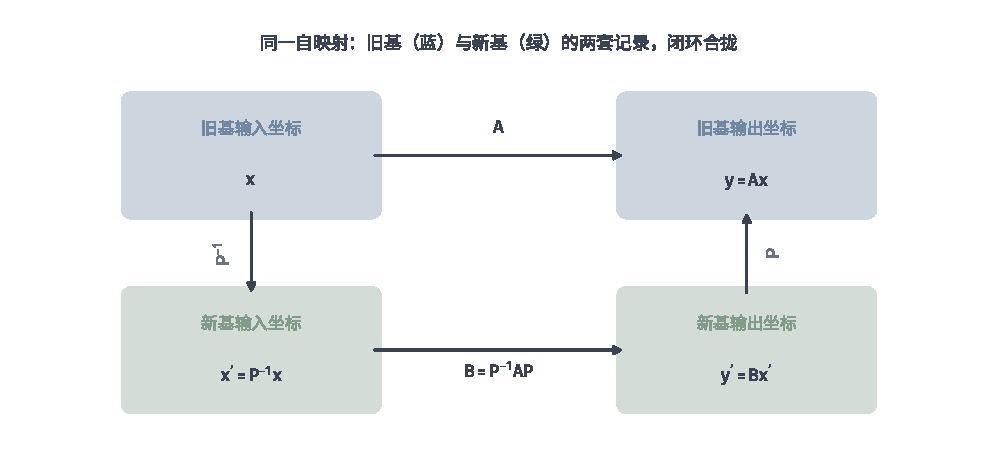
\includegraphics[width=169mm]{figures/01-mathematical-preliminaries-upper/02-linear-spaces/matplotlib/ls-similarity-change-of-basis-flow/ls-similarity-change-of-basis-flow.pdf}
  \caption{相似换基的闭环。上边是旧基下的作用$\bm y=\bm A\bm x$；左边箭头把旧输入
  坐标$\bm x$换成新输入坐标$\bm x'=\bm P^{-1}\bm x$，下边是新基下的作用
  $\bm y'=\bm B\bm x'=\bm P^{-1}\bm A\bm P\,\bm x'$，右边箭头把新输出坐标
  换回旧读数$\bm y=\bm P\bm y'$。两条路径给出同一个$\bm y$，闭环合拢即
  $\bm B=\bm P^{-1}\bm A\bm P$。}
  \label{fig:ls-similarity-change-of-basis-flow}
\end{figure*}

用一次具体换基核对对象未变，按首次阅读的顺序一步步代入。第一步选基并排换基
矩阵：在$\mathbb R^2$中取旧基为标准基，新基为$\bm b_1'=\bm e_1$、
$\bm b_2'=\bm e_1+\bm e_2$；新基向量在旧基下的坐标分别是
$(1,0)^{\top}$与$(1,1)^{\top}$，排成列得
$\bm P=\begin{bmatrix}1&1\\0&1\end{bmatrix}$，所以旧坐标$\bm x=\bm P\bm x'$，
反向为$\bm P^{-1}=\begin{bmatrix}1&-1\\0&1\end{bmatrix}$。

第二步写出旧基记录的映射。设旧矩阵为$\bm A=\begin{bmatrix}2&1\\0&3\end{bmatrix}$，
它满足$T\bm e_1=2\bm e_1$、$T\bm e_2=\bm e_1+3\bm e_2$。第三步代入公式
计算新记录：
\[
 \bm B=\bm P^{-1}\bm A\bm P
 =\begin{bmatrix}1&-1\\0&1\end{bmatrix}
 \begin{bmatrix}2&1\\0&3\end{bmatrix}
 \begin{bmatrix}1&1\\0&1\end{bmatrix}
 =\begin{bmatrix}2&0\\0&3\end{bmatrix}.
\]

两种记录对应同一个$T$：新基的两个方向$\bm e_1$与$\bm e_1+\bm e_2$正好是
$T$的两个特征方向，$T$把它们分别放大$2$倍与$3$倍，换到新基后系数可直接读出，
正是$\bm B$的对角元。改变的只是沿哪两条基方向读取，$T$本身没有被改写。

\subsubsection{性质与不变量}
\label{sec:ls-similarity-properties}

为什么先要核对相似是等价关系？换基可以做多次：不换基对应自己，换基两次可以
原路换回，两次换基可以合并成一次。具体写下来：$\bm A=\bm I^{-1}\bm A\bm I$
给出自反性；由$\bm B=\bm P^{-1}\bm A\bm P$得
$\bm A=\bm P\bm B\bm P^{-1}$给出对称性；若$\bm B=\bm P^{-1}\bm A\bm P$、
$\bm C=\bm Q^{-1}\bm B\bm Q$，则
$\bm C=(\bm P\bm Q)^{-1}\bm A(\bm P\bm Q)$给出传递性。

换基怎样搬动核与像，由这个公式直接读出。$\bm B\bm x'=\bm0$当且仅当
$\bm A(\bm P\bm x')=\bm0$，即$\bm P\bm x'\in\ker\bm A$，故
$\ker\bm B=\bm P^{-1}\ker\bm A$；同理
$\operatorname{im}\bm B=\bm P^{-1}\operatorname{im}\bm A$。核与像作为
方向集合被可逆坐标对应整体搬运，并不是逐点保持在原坐标位置。

可逆坐标对应是线性双射，保持维数，因此
\begin{equation}
 \operatorname{rank}\bm B=\operatorname{rank}\bm A,
 \qquad
 \dim\ker\bm B=\dim\ker\bm A.
 \label{eq:ls-similarity-invariants}
\end{equation}
这是本章能直接给出的相似不变量；迹与行列式在运算章定义后再核对它们的相似
不变性。

复合作用在换基下同样良好行为，这对反复作用很重要。若
$\bm B_1=\bm P^{-1}\bm A_1\bm P$、$\bm B_2=\bm P^{-1}\bm A_2\bm P$，则
\begin{equation}
 \bm B_1\bm B_2
 =\bm P^{-1}\bm A_1\bm P\,\bm P^{-1}\bm A_2\bm P
 =\bm P^{-1}\bm A_1\bm A_2\bm P.
 \label{eq:ls-similarity-product}
\end{equation}
中间的$\bm P\bm P^{-1}$抵消，复合仍表示同一对映射的复合；由此归纳得
$\bm B^k=\bm P^{-1}\bm A^k\bm P$，反复作用在新基下仍是同一过程的记录。

相应核的维数等信息保留，但一般换基不保持原坐标下的欧氏长度与夹角；长度、
夹角属于内积与度量，本章不作要求。

\subsubsection{成立条件}
\label{sec:ls-similarity-conditions}

把$\bm B=\bm P^{-1}\bm A\bm P$两端左乘$\bm P$，相似等价改写为关于
$\bm P$的方程
\begin{equation}
 \bm A\bm P=\bm P\bm B.
 \label{eq:ls-similarity-equation}
\end{equation}
这是关于$\bm P$各元素的一组线性约束。方程有非零解还不够，必须再筛出可逆解
$\det\bm P\neq0$（行列式在运算章定义）：只找到非零但奇异的$\bm P$，得到的
只是两个坐标子空间之间的对应，不是两组基之间的换基。若找到可逆$\bm P$满足
上式，则$\bm B=\bm P^{-1}\bm A\bm P$，按新基恢复出的映射与$\bm A$记录的
是同一个$T$：新坐标经$\bm B$作用后，由$\bm P$换回旧坐标恰为$\bm A$的作用。

反过来说，秩、核维数相同只给必要条件，不足以判定相似。例如$\bm I_2$与
$\begin{bmatrix}1&1\\0&1\end{bmatrix}$同秩、同核维数（核均为零），但
$\ker(\bm I_2-\bm I_2)=\mathbb R^2$与
$\ker\left(\begin{bmatrix}0&1\\0&0\end{bmatrix}\right)$维数不同，因而不相似。
检查$T$减去某个数值作用后的核维数，是比总秩更细的必要条件；完整判据需要后续
分解工具。把相似化为简单标准形的完整分类，依赖特征方向与实分裂等后续概念，在
幂序列与长期行为一节回接；本章只承诺定义层面的换基验证和已建立不变量的必要性，
不把相同秩或相同数值特征当作充分条件。

\subsection{相抵}
\label{sec:ls-equivalence-matrices}

\subsubsection{定义与含义}
\label{sec:ls-equivalence-meaning}

与同一空间上的相似对照，这里处理一般线性映射$T:V\to W$，输入空间$V$（维数$d$）
与输出空间$W$（维数$m$）是两个不同空间，各自选择自己的基，两端不必由同一个
换基矩阵联系。当$d\neq m$时甚至无法用同一个方阵同时充当两次换基，这正是相抵
比相似更一般的原因；矩阵可以是长方形$\bm A\in\mathbb R^{m\times d}$。贯穿例
$T_\varepsilon:\mathbb R^2\to\mathbb R^3$（系数映射为三个样本拟合值）正是这种两端
不同维的映射，输入端选系数基、输出端选样本读取基，各自独立。

输入端在$V$内换基，旧坐标$\bm x=\bm P\bm x'$，$\bm P$是$d\times d$可逆矩阵，
记录输入基的更换。把它代入映射$\bm y=\bm A\bm x$时，$\bm P$出现在$\bm A$的
右侧：$\bm A\bm P\bm x'$，先完成输入坐标的换算，再进入作用。输出端在$W$内
独立换基，旧坐标$\bm y=\bm Q\bm y'$，$\bm Q$是$m\times m$可逆矩阵，记录
输出基的更换。要求出新坐标$\bm y'$，就要在等式左侧用$\bm Q^{-1}$把旧输出
坐标解开，$\bm Q^{-1}$出现在$\bm A$的左侧。两端的$\bm P,\bm Q$彼此独立，
不要求对方是可逆方阵之外的任何关系。

\paragraph{相抵变换的推导}
把两次代入$\bm y=\bm A\bm x$，得$\bm Q\bm y'=\bm A\bm P\bm x'$，左乘
$\bm Q^{-1}$后
\begin{equation}
 \bm y'=\bm Q^{-1}\bm A\bm P\,\bm x',
 \qquad\text{即}\qquad
 \bm B=\bm Q^{-1}\bm A\bm P.
 \label{eq:ls-equivalence-transform}
\end{equation}
若存在实可逆$\bm Q\in\mathbb R^{m\times m}$与$\bm P\in\mathbb R^{d\times d}$
使上式成立，就称同形的$\bm A,\bm B$
\term{相抵}（equivalent matrices）。

右乘可逆$\bm P$对应输入基（列方向）的更换，左乘可逆$\bm Q^{-1}$对应输出基
（行方向）的更换。初等列变换与初等行变换分别是两端换基的具体实现，行列操作
由此获得坐标含义，不只是数表上的算术动作。

图~\ref{fig:ls-equivalence-two-sided-bases-flow}把两端独立换基的闭环画出来：
输入端经$\bm P^{-1}$换基，输出端经$\bm Q^{-1}$换基，新基下的作用$\bm B$夹在
两次回换之间。沿上边直接用$\bm A$作用，与沿下边“输入换基—作用$\bm B$—输出
回换”，殊途同归；闭环合拢的条件正是$\bm B=\bm Q^{-1}\bm A\bm P$。与
图~\ref{fig:ls-similarity-change-of-basis-flow}对照可以看出，相似是左右
两侧共用同一个$\bm P$的特例。
\begin{figure*}[htbp]
  \centering
  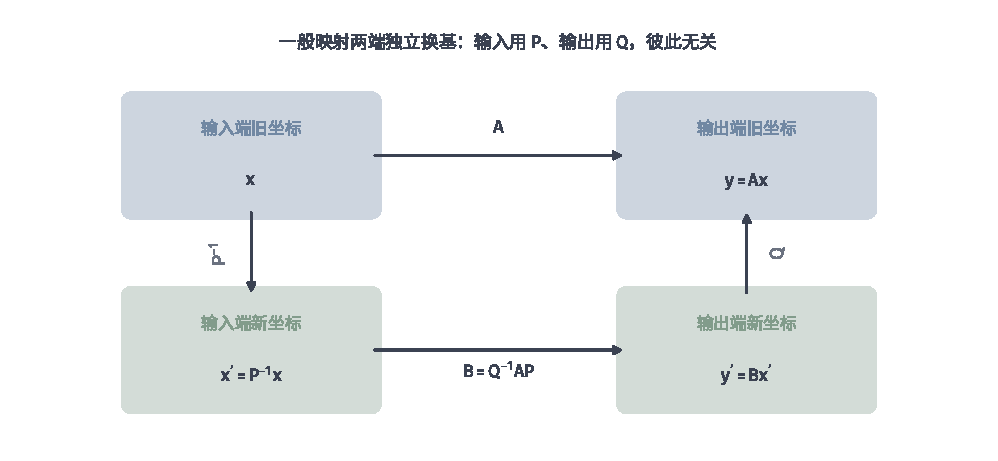
\includegraphics[width=169mm]{figures/01-mathematical-preliminaries-upper/02-linear-spaces/matplotlib/ls-equivalence-two-sided-bases-flow/ls-equivalence-two-sided-bases-flow.pdf}
  \caption{相抵两端换基的闭环。上边是旧坐标下的作用$\bm y=\bm A\bm x$；左边箭头
  把输入旧坐标$\bm x$换成新坐标$\bm x'=\bm P^{-1}\bm x$，右边箭头把输出新坐标
  $\bm y'$换回旧读数$\bm y=\bm Q\bm y'$，下边是新基下的作用
  $\bm y'=\bm B\bm x'=\bm Q^{-1}\bm A\bm P\,\bm x'$。两端的$\bm P$与$\bm Q$
  彼此独立；闭环合拢即$\bm B=\bm Q^{-1}\bm A\bm P$。}
  \label{fig:ls-equivalence-two-sided-bases-flow}
\end{figure*}

\subsubsection{性质与不变量}
\label{sec:ls-equivalence-properties}

相抵是不是等价关系，同样由公式直接核对。自反取$\bm Q=\bm I,\bm P=\bm I$得
$\bm A=\bm I^{-1}\bm A\bm I$。对称：由$\bm B=\bm Q^{-1}\bm A\bm P$，左乘
$\bm Q$、右乘$\bm P^{-1}$得$\bm A=\bm Q\bm B\bm P^{-1}$，形式仍为两端可逆
夹乘。传递：若$\bm B=\bm Q_1^{-1}\bm A\bm P_1$、
$\bm C=\bm Q_2^{-1}\bm B\bm P_2$，代入得
$\bm C=(\bm Q_1\bm Q_2)^{-1}\bm A(\bm P_1\bm P_2)$，两端可逆矩阵分别复合。

换基对核与像的影响两端各自独立。由\eqref{eq:ls-equivalence-transform}
$\bm B=\bm Q^{-1}\bm A\bm P$，$\bm B\bm x'=\bm0$等价于$\bm A\bm P\bm x'=\bm0$，
即$\bm P\bm x'\in\ker\bm A$，故$\ker\bm B=\bm P^{-1}\ker\bm A$；而
$\bm B\bm x'=\bm Q^{-1}(\bm A\bm P\bm x')$，$\bm P$遍历输入使
$\bm A\bm P\bm x'$遍历$\operatorname{im}\bm A$，$\bm Q^{-1}$再搬到输出端，
故$\operatorname{im}\bm B=\bm Q^{-1}\operatorname{im}\bm A$。核在输入端被
$\bm P$搬运，像在输出端被$\bm Q$搬运。

两次可逆坐标对应都保持维数，因此
\begin{equation}
 \operatorname{rank}\bm B=\operatorname{rank}\bm A,
 \qquad
 \dim\ker\bm B=d-\operatorname{rank}\bm A,
 \qquad
 m-\dim\operatorname{im}\bm B=m-\operatorname{rank}\bm A.
 \label{eq:ls-equivalence-invariants}
\end{equation}
保持的是两端方向的独立个数，不能宣称原坐标中的核或像逐点不动。

两端坐标独立改变，也不保留与某一端特定坐标有关的长度、角度等数值信息；相抵
比相似允许的记录变化更宽，度量由运算章的内积与范数规定。还须注意，输入与输出
是不同空间时，$\bm B$无法对自身重复作用，“复合”只发生在同一空间的自映射
之间；这是相抵与相似在对象上的根本区别。

\subsubsection{成立条件}
\label{sec:ls-equivalence-conditions}

构造判据之前，先在两端各选一组配合$T$的基。取$\ker\bm A$的一组基并扩充为
$V$的基：新增的$r$个方向在核外，它们的像线性无关（否则某一非零组合的像为零，
该组合就落进核），并恰好张成$\operatorname{im}\bm A$；在$W$中把这组$r$个
像扩充为输出基，余下的$m-r$个基方向上没有可达输出。在这样选取的输入基与输出基
下，矩阵化为秩标准形
\begin{equation}
 \begin{bmatrix}\bm I_r&\bm0\\\bm0&\bm0\end{bmatrix},
 \qquad r=\operatorname{rank}\bm A,
 \label{eq:ls-rank-normal-form}
\end{equation}
其中$r$个独立输入方向被送到$r$个独立输出方向，其余方向进核、其余输出为缺失。

\paragraph{同形同秩矩阵的相抵判据}
\begin{theorem}[相抵判据]
\label{thm:ls-equivalence-criterion}
两个同形实矩阵$\bm A,\bm B\in\mathbb R^{m\times d}$相抵，当且仅当
$\operatorname{rank}\bm A=\operatorname{rank}\bm B$。
\end{theorem}
必要性由两端可逆保持秩得到；充分性由二者都化为同一个秩标准形
\eqref{eq:ls-rank-normal-form}，两次化简连接为$\bm Q^{-1}\bm A\bm P$。固定
形状之后，秩就是相抵的完整不变量。设$\bm A,\bm B$都化到同一秩标准形$\bm R$：
$\bm R=\bm Q_A^{-1}\bm A\bm P_A=\bm Q_B^{-1}\bm B\bm P_B$。两式对接得
$\bm B=\bm Q_B\bm Q_A^{-1}\bm A\bm P_A\bm P_B^{-1}$，对照
\eqref{eq:ls-equivalence-transform}即解出$\bm Q=\bm Q_A\bm Q_B^{-1}$、
$\bm P=\bm P_A\bm P_B^{-1}$。具体用哪些消元或分解把矩阵化到标准形，算法在
求解章建立，这里只给出对接关系。退化边界也由此清楚：零秩对应零映射，
$\bm A=\bm0$只能与零矩阵相抵；满行秩时输出全部可达，满列秩时核为零。同秩
但不同形状的矩阵不直接比较，相抵以同形为前提。

\subsection{合同}
\label{sec:ls-congruence}

\subsubsection{定义与含义}
\label{sec:ls-congruence-meaning}

前两种关系记录单输入算子；合同记录的是把两个向量位置分别读成一个数的规则。
\term{双线性型}（bilinear form）是在两个输入位置上分别保持线性组合的规则
$B:V\times V\to\mathbb R$，即$B(a\bm u+b\bm u',\bm v)=aB(\bm u,\bm v)+bB(\bm u',\bm v)$，
另一位置同理。在选定基下它写成$B(\bm u,\bm v)=\bm u^{\top}\bm A\bm v$，矩阵
$\bm A$记录这次读取：$A_{i,j}=B(\bm b_i,\bm b_j)$。例如$B(\bm u,\bm v)=u_1v_2$
由$\bm A=\begin{bmatrix}0&1\\0&0\end{bmatrix}$记录，对象不是一个自映射，
$\bm A$乘的是两个变量而不是把一个向量送到另一个向量。

双线性型的两个位置都取自同一个空间$V$，因此换基时两个位置使用同一组变量、
同一次坐标更换：$\bm u=\bm P\bm x$，$\bm v=\bm P\bm y$，$\bm P$是同一个
可逆换元矩阵，而不是左右各取一个。这与相抵形成对照：相抵的输入、输出是两个空间，
两侧可以分别换基；合同只在一个空间内换元，若给两个位置各配一个不同矩阵，就是在
两套互不相干的坐标里读取同一个型，不再记录换元前后的同一个$B$。

\paragraph{合同变换的推导}
代入得
\begin{equation}
 B(\bm P\bm x,\bm P\bm y)
 =\bm x^{\top}\bm P^{\top}\bm A\bm P\,\bm y,
 \qquad\text{即}\qquad
 \bm C=\bm P^{\top}\bm A\bm P.
 \label{eq:ls-congruence-transform}
\end{equation}
若存在实可逆$\bm P$使上式成立，就称$\bm A$与$\bm C$
\term{合同}（congruent）。合同本身不要求$\bm A$对称。

把两个位置取成同一个变量，$q_A(\bm x)=\bm x^{\top}\bm A\bm x$称为
\term{二次型}（quadratic form）。
只有对称部分$\bm S=(\bm A+\bm A^{\top})/2$出现在$q_A$中：
$\bm x^{\top}\bm A\bm x=\bm x^{\top}\bm S\bm x$，反对称部分取值恒为零。
一般双线性型与其二次型不能混同，非对称矩阵的反对称信息在对角取值中消失。合同与
相似的对象也由此分清：合同记录同一个二次型或双线性读取在换元下的表达，变换是
$\bm P^{\top}$；相似记录同一个自映射在换基下的表达，变换是$\bm P^{-1}$。
即使形式上都乘可逆矩阵，二者回答的问题不同。

\subsubsection{性质与不变量}
\label{sec:ls-congruence-properties}

合同是不是等价关系，由$\bm C=\bm P^{\top}\bm A\bm P$核对。自反取
$\bm P=\bm I$得$\bm A=\bm I^{\top}\bm A\bm I$。对称：两边乘
$\bm P^{-\top}$与$\bm P^{-1}$（其中$\bm P^{-\top}=(\bm P^{-1})^{\top}$），
得$\bm A=\bm P^{-\top}\bm C\bm P^{-1}$。传递：若
$\bm C=\bm P_1^{\top}\bm A\bm P_1$、$\bm D=\bm P_2^{\top}\bm C\bm P_2$，
代入得$\bm D=(\bm P_1\bm P_2)^{\top}\bm A(\bm P_1\bm P_2)$，两个可逆
换元复合后仍可逆。

换元怎样改变二次型的取值，是合同真正要回答的问题。由
$q_C(\bm y)=\bm y^{\top}\bm C\bm y
=(\bm P\bm y)^{\top}\bm A(\bm P\bm y)=q_A(\bm P\bm y)$，
可逆换元把$q_A$在$\bm P\bm y$方向上的取值搬到$q_C$在$\bm y$方向上。因为
$\bm P$可逆，$\bm y\neq\bm0$当且仅当$\bm P\bm y\neq\bm0$，于是
$q_A(\bm P\bm y)>0$、$=0$、$<0$分别对应$q_C(\bm y)>0$、$=0$、$<0$；
数值大小随换元改变，正负号与零值方向双向对应保持。

对所有非零$\bm x$都有$q_A(\bm x)>0$时称\term{正定}（positive definite），
$q_A(\bm x)\geq0$时称\term{半正定}（positive semidefinite），既取正值又取
负值时称\term{不定}（indefinite）。可逆换元下正、负、零值方向双向对应，
因此这些符号性质保持；以使二次型严格为正或严格为负的最大子空间维数，以及
$\dim\ker\bm A$，记录符号结构，它们都经可逆换元给出的线性双射保持不变，
秩也因$\bm P$可逆而保持。这里用二次型本身判断符号，不借用尚未建立的谱分类。

还须区分两类“零”：$q_A(\bm x)=0$不等于$\bm A\bm x=\bm0$。例如$q=x^2-y^2$
在$(1,1)^{\top}$上取值为零，但$\operatorname{diag}(1,-1)$可逆、核为零；
零能量方向不是核方向，不能从某个方向的零能量判定零惯性。

\subsubsection{成立条件}
\label{sec:ls-congruence-conditions}

验证两个矩阵合同，就是寻找可逆$\bm P$使$\bm C=\bm P^{\top}\bm A\bm P$；这是
关于$\bm P$元素的一组方程，可逆性是合法换元的前提。秩相同只给出必要条件：可逆
$\bm P$保秩，合同必有同秩，但同秩不足以判定合同，例如$\operatorname{diag}(1,1)$
与$\operatorname{diag}(1,-1)$同秩，正负方向个数不同，并不合同。能直接配方的
例子可以当场看出符号：$x^2+2xy+y^2=(x+y)^2$恒非负、在$x+y=0$上取零，是
半正定；$x^2-y^2=(x+y)(x-y)$在$(1,0)$取正、在$(0,1)$取负，是不定；
$x^2$只取非负且仅在$x=0$取零。配方把二次型拆成若干带符号的平方项，可逆换元
不改变正、负平方项的个数，故配方直接处理的符号结构在可逆换元下保持。

实对称矩阵合同的完整判据（正负零方向个数相同，即惯性三元组）需要把正、负、零方向
化为相同标准坐标，其构造在二次优化一节以谱为工具完成；本章只由可逆对应证明符号
子空间维数保持，不提前用特征值定义惯性或承诺完整分类。同惯性的充要分类也不扩大
到任意非对称矩阵：反对称部分不出现在二次型中，非对称双线性型不能套用实对称型的
判据；正定情形只含正方向，因此同阶正定二次型彼此合同。

\section{本章小结}
\label{sec:ls-representation-summary}

本章回答“怎样表示”，得到一条由对象到记录的链条。4.1先辨认标量、向量、矩阵与
张量：对象本身不是一串数，数只是选定方向以后的记录。4.2把可相加、可缩放的对象
规定为实线性空间，张成回答表示能否存在，线性无关回答表示是否唯一，二者共同给出
基与不依赖选择的维数。4.3研究同一环境中子空间的包含、交、和与直和，维数公式
\eqref{eq:ls-dimension-formula}由公共基扩充得到，一般补空间不是正交补。

4.4固定有序基建立坐标，并区分被动换基与主动作用。4.5把保持线性组合的对应记录为
矩阵，用核、像与秩零度定理\eqref{eq:ls-rank-nullity}计数被消去与被保留的
自由度，据此判断单射、满射与可逆性。4.6把标量读取规则收集为对偶空间，对偶映射
以转置表示，并由此证明行秩等于列秩。4.7以差属于子空间定义等价类，商空间消去指定
方向，且$V/\ker T\cong\operatorname{im}T$。

4.8比较三种换记录关系：相似$\bm B=\bm P^{-1}\bm A\bm P$记录同一自映射，
相抵$\bm B=\bm Q^{-1}\bm A\bm P$记录两端独立换基的同一映射，合同
$\bm C=\bm P^{\top}\bm A\bm P$记录同一双线性读取；三者对象不同，保持的
不变量也不同，且本章只用秩与核维数。

仅有坐标尚未指定长度、夹角或最优性：度量配对与范数在运算章建立，反求未知量在
求解章按目标判存在唯一，结果对数据与计算误差的敏感度在分析章衡量。贯穿例
$\bm X_\varepsilon$的近共线结构，将在这些章节依次回到拟合稳定而系数敏感的
现象。
